\documentclass[journal]{IEEEtran}

\usepackage[usenames,dvipsnames,svgnames,table]{xcolor}
\usepackage{amsmath}
\usepackage{amsfonts}
\usepackage{cite}
\usepackage{graphicx}
\usepackage{listings}
\usepackage{multirow}
\usepackage{tabularx}
\usepackage{varioref}
\usepackage{hyperref}
\usepackage[noabbrev,capitalize]{cleveref}
\usepackage[group-separator={,}, group-four-digits=true]{siunitx}
\usepackage{lscape}
\usepackage{bm}
\usepackage{chngpage}
\usepackage{blindtext} % For filler text

\usepackage[english]{babel}
\usepackage[utf8]{inputenc}

%Includes "References" in the table of contents
\usepackage[nottoc]{tocbibind}


\lstset{
  frame=single,
  basicstyle=\ttfamily,% print whole listing small
  language=R,
  aboveskip=3mm,
  belowskip=3mm,
  showstringspaces=false,
  columns=flexible,
  numbers=none,
  commentstyle=\color{ForestGreen},
  stringstyle=\color{Maroon},
  breaklines=true,
  breakatwhitespace=true,
  tabsize=2,
  literate={<-}{{$\gets$}}1 {~}{{$\sim$}}1
}

\hypersetup{
  colorlinks=true,
  linkcolor=blue,
  urlcolor=blue,
}

\sisetup{output-exponent-marker=\textsc{e}}

\begin{document}

\title{Facial Keypoints Detection}
\author{Will Clark and Matthew DeLio\\
University of Chicago Booth School of Business\\
\textsf{\{will.clark,mdelio\}@chicagobooth.edu}}

% The paper headers
\markboth{Machine Learning (BUS 41201) Final Project}
{Machine Learning (BUS 41204) Final Project}

\maketitle

\section{Introduction}\label{intro}

\subsection{Problem Summary}

The goal of this paper is to predict the $(x,y)$ coordinates of 15 facial keypoints for a given set of 96-by-96 grayscale images. The keypoints are:
\begin{itemize}
\item Left and right eye center (2)
\item Left and right eye inner and outer corners (4)
\item Left and right eyebrow inner and outer ends (4)
\item Nose tip (1)
\item Mouth left and right corner (2)
\item Mouth top and bottom lip center (2)
\end{itemize}
A random sample of images and the associated keypoints are shown for reference in \cref{fig:random_faces}. Note that of the displayed faces, only two have the full set of keypoints plotted. This is a feature of the data, namely, that most faces are missing at least multiple keypoints. Accordingly, we predict two values for each keypoint: (1) whether it is present in an image or not, and (2) what its $(x,y)$ coordinates would be if it were present.raining

There are 7049 images in the training set provided by Kaggle. We randomly subset the data so that 70 percent of images are for training a model and the other 30 percent are for validation. There is also a true test set of 1783 images for which we only have the image data but not the keypoint data. This is the set on which the Kaggle contest is judged.

The criterion for model accuracy (and evaluation in the Kaggle contest) is the root means square error of all keypoint coordinates:
\[ \text{RMSE}=\sqrt{\frac{1}{n} \sum_{i=1}^{n} \left( y_i - \hat{y}_i\right)^2} \]

\begin{figure}[!ht]
  \centering
  \caption{Random Sub-Sample of Faces and Keypoints}
  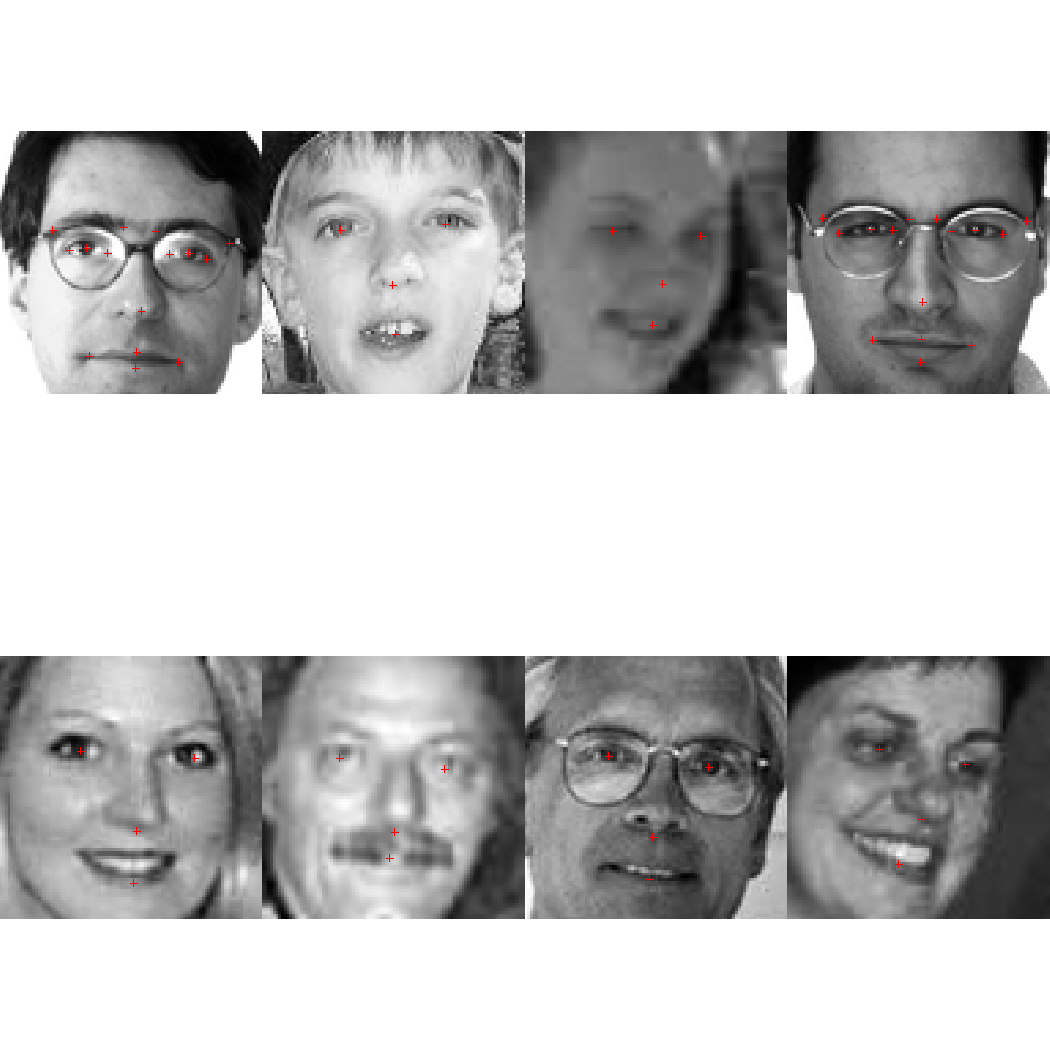
\includegraphics[scale=.49]{random_faces.pdf}
  \label{fig:random_faces}
\end{figure}

\subsection{Data}

As discussed in \cref{intro}, most images do not contain all keypoints, which presents a problem when we are trying to train our model. One naive solution would be to throw out all faces without all keypoints, but doing so would remove 4909 images from our training data set (out of 7049 total images)--about 70 percent of our data.

An important observation is that keypoints tend to be missing in groups, so that (as an example) if an image does not have one of the eyebrow keypoints, it tends to also not have all other eyebrow keypoints. Accordingly, we bundle the keypoints into the following groups (the number of images containing all keypoints in the group are reported in parentheses):
\begin{itemize}
\item eye center: left eye center, right eye center (7033)
\item eye corner: left eye inner corner, left eye outer corner, right eye inner corner, right eye outer corner (2247)
\item eyebrow: left eyebrow inner end, left eyebrow outer end, right eyebrow inner end, right eyebrow outer end (2190)
\item mouth (bottom): mouth center bottom lip (7016)
\item mouth (excl. bottom): mouth left corner, mouth right corner, mouth center top lip (2260)
\item nose: nose tip (7049)
\end{itemize}
For each feature, then, we can group it with other features that tend to be present in the same image. Within a group, we throw out images in which all keypoints \textit{in that group} are not present, but in 22 out of 30 cases this requires us to remove less than 1 percent of the available images (in the other 8 cases, we throw out between 1 and 4 percent of available images).

Splitting the features into groups like this requires that we train six models, but each model will have more available training data than a single model required to predict all features. 

A related point is that we will also need to predict whether or not a keypoint is contained in a feature, so that we can predict an empty value for keypoints that are likely to be missing in the test set. We discuss this model more fully in \cref{missing}.

\subsection{Tools and Software}

The main tool we use in this paper is a multilayer convolutional neural network. We built and trained the model in Python using the Theano and Lasagne libraries.\footnote{Lasagne is "a lightweight library to build and train neural networks in Theano." See \url{https://github.com/Lasagne/Lasagne} for details.} One advantage of this technology stack is that computation can be carried out on a graphics card (GPU) which can significantly improve calculation speed.

To take advantage of Theano's GPU capability, we set up our computing environment using a g2.2xlarge EC2 instance from Amazon Web Services. Doing so gave us access to an NVIDIA GPUs with 1536 CUDA cores that performed the bulk of the calculation. In our case, the performance improvement from utilizing the g2.2xlarge instance (compared to running locally) was approximately 40x.

\section{Missing Feature Model}\label{missing}

Since the data contain many missing features caused in some cases by partially obscured images and just poor labelling, our resulting model must also predict the presence of features.  To predict this we turn to a slightly modified version of the neural network described in \cref{neural} with a sigmoid non-linearity on the output layer and the binary cross-entropy loss function defined below:

\[\label{eq:bin_cross}
 L = -target \log(p) - (1 - target) \log(1 - p)
\]
where \texttt{target} indicates whether the feature is actually missing ($\in \{0,1\}$) and \texttt{p} is the predicted probability of the feature being missing

For many of the features (see \cref{fig:logistic_boxplots_eye,fig:logistic_boxplots_eyebrow,fig:logistic_boxplots_mouth}, the neural network does a good job separating the two classes and producing probabilities that make logical sense.  The ones that it doesn't separate well, like \texttt{Left Eye Center}, \texttt{Right Eye Center} and \texttt{Mouth Center Bottom Lip}, have few missing data-point exemplars in the training data (9, 9, and 23 respectively out of 4934 samples).

\begin{figure}[!ht]
  \centering
  \caption{Boxplots for Missing Eye Features}
  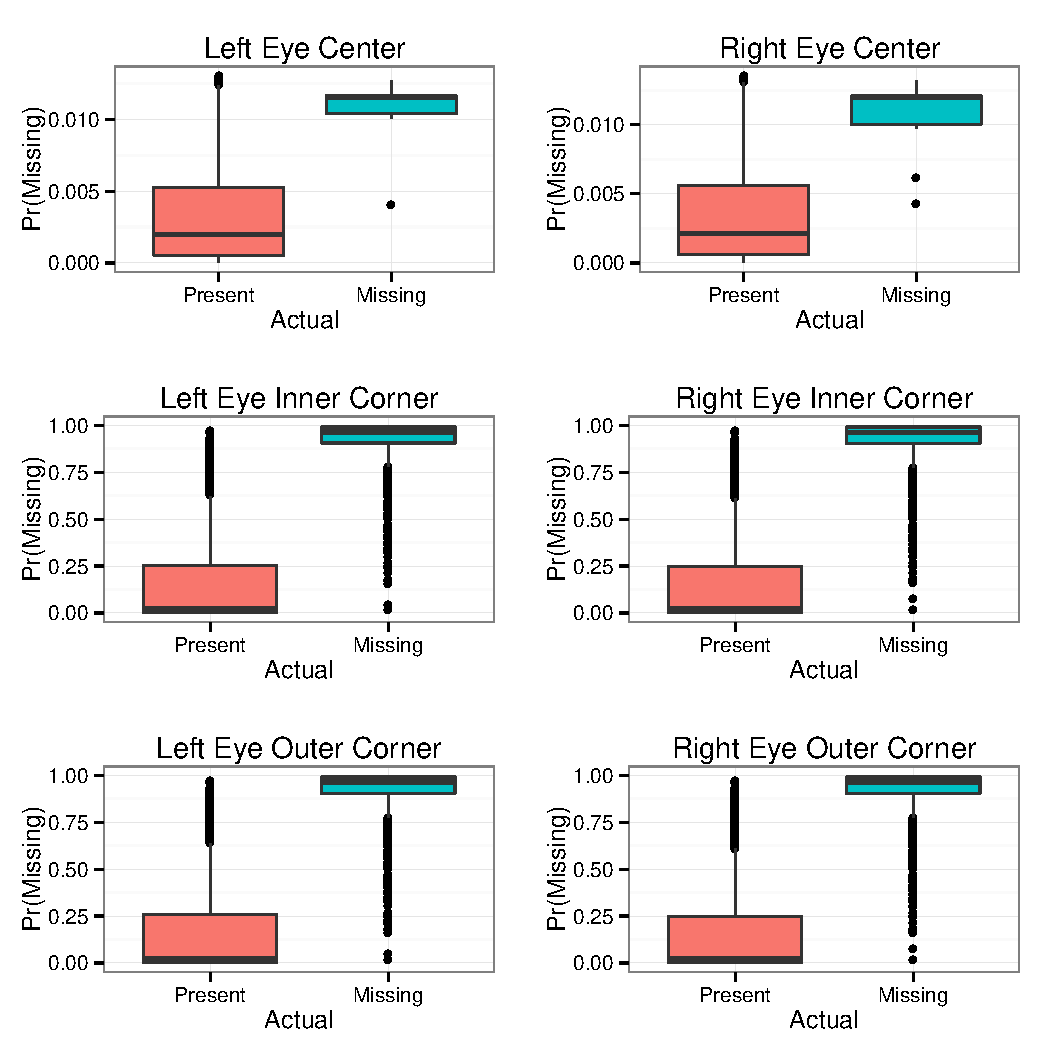
\includegraphics[scale=.49]{logistic_boxplots_eye.pdf}
  \label{fig:logistic_boxplots_eye}
\end{figure}

% We can probably drop these next two, they don't add much to the discussion...maybe we can just mention they they look identical (throw them in an appendix)
\begin{figure}[!ht]
  \centering
  \caption{Boxplots for Missing Eyebrow Features}
  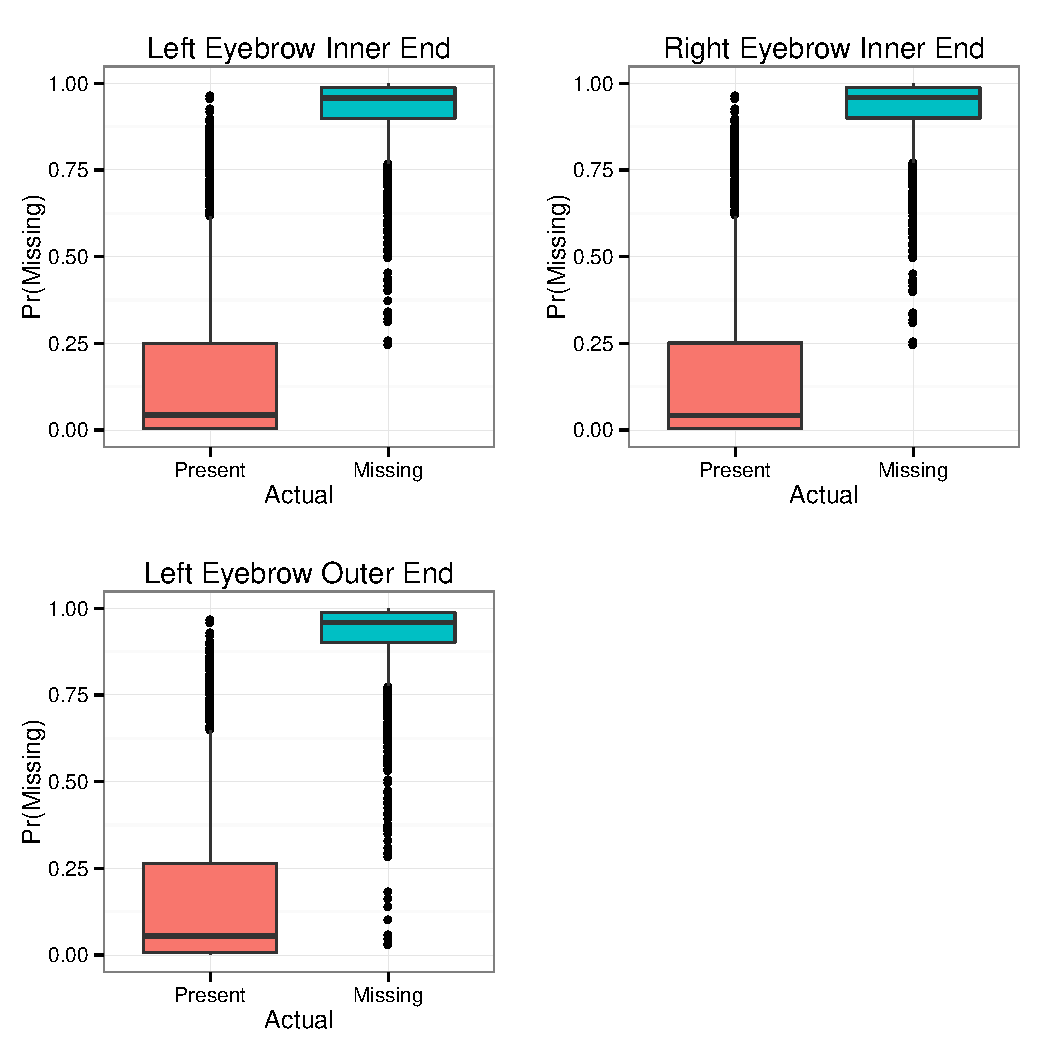
\includegraphics[scale=.49]{logistic_boxplots_eyebrow.pdf}
  \label{fig:logistic_boxplots_eyebrow}
\end{figure}

\begin{figure}[!ht]
  \centering
  \caption{Boxplots for Missing Mouth Features}
  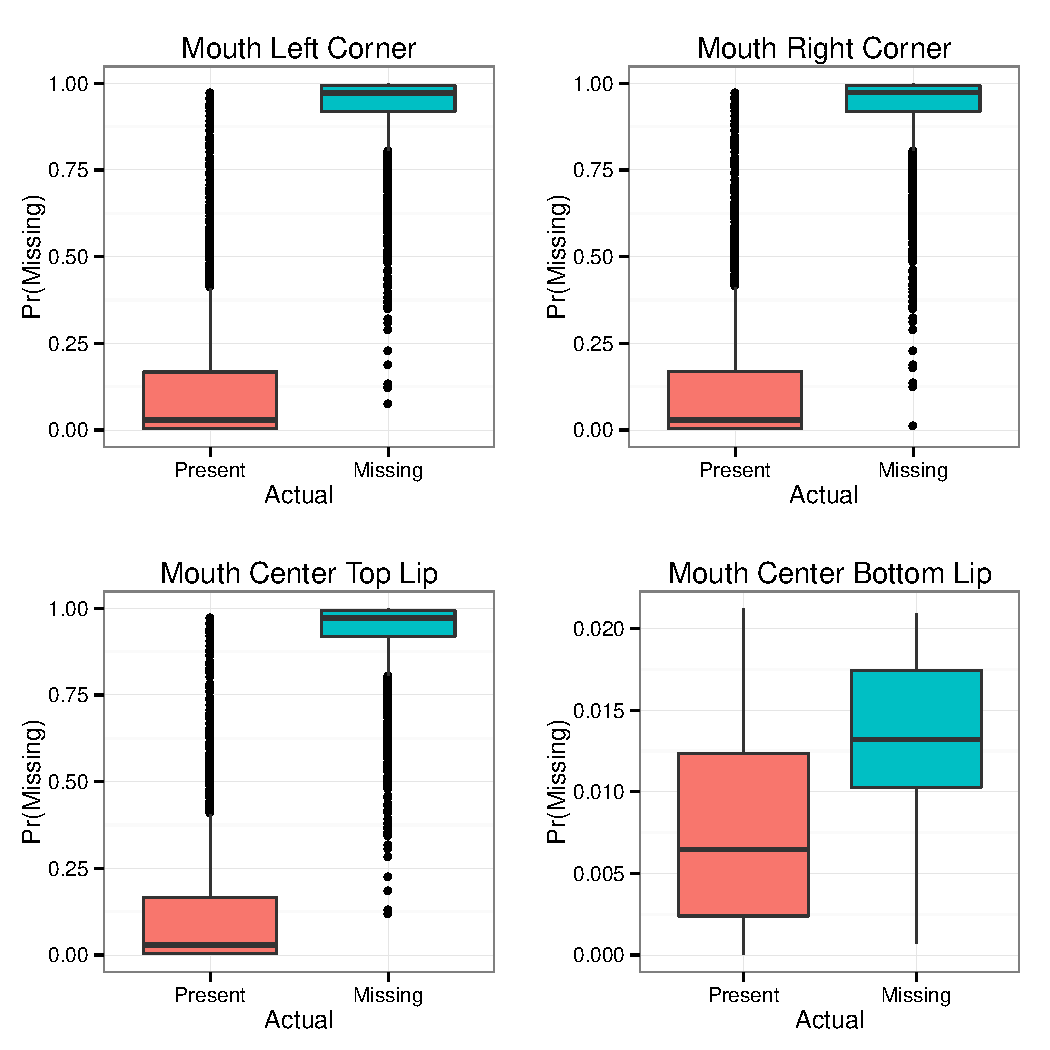
\includegraphics[scale=.49]{logistic_boxplots_mouth.pdf}
  \label{fig:logistic_boxplots_mouth}
\end{figure}

% \begin{figure}[!ht]
%   \centering
%   \caption{Boxplots for Missing Nose Feature}
%   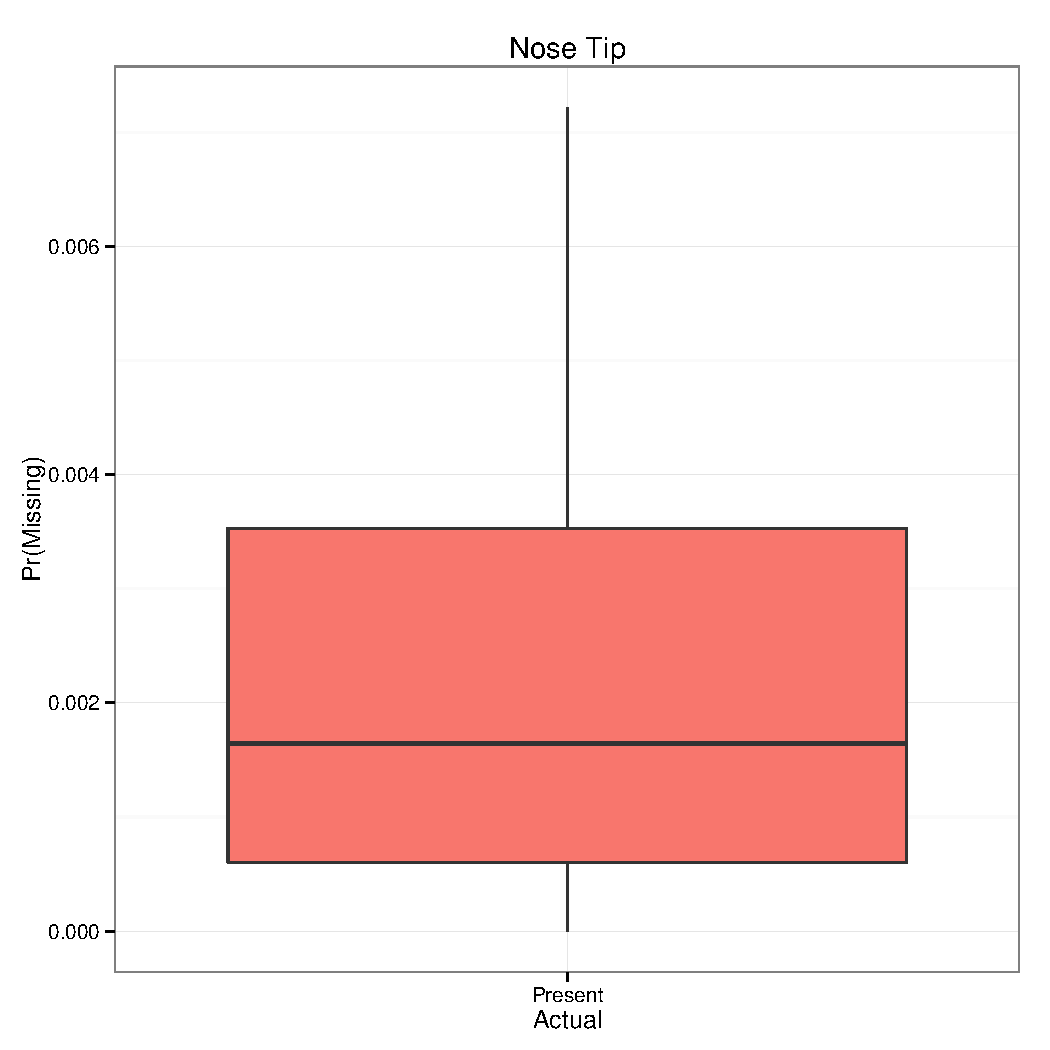
\includegraphics[scale=.49]{logistic_boxplots_nose.pdf}
%   \label{fig:logistic_boxplots_nose}
% \end{figure}

With the output trained, we next turn to determining the optimal cutoff.  Using the R package \texttt{OptimalCutpoints} we choose to maximize the accuracy area \cite{lewis2008use,greiner1995two,greiner1996two} which is defined in \cref{eq:roc_aa}.

\[\label{eq:roc_aa}
AA(c)=\frac{TP(c)TN(c)}{(TP(c)+FN(c))(FP(c)+TN(c))}
\]
where $TP$ = True Positives, $TN$ = True Negatives, $FN$ = False Negatives, \& $FP$ = False Positives

Looking over our boxplots, we see there are generally two categories of features: those that are missing often and those that are not.  For the ones that are missing often, we have a relatively good separability between the predicted probabilities.  For those that are not missing often, our predictive power diminishes.  Turning to the ROC plot for a feature that is missing quite often, \texttt{Left Eye Inner Corner}, (see \cref{fig:roc_left_eye_inner_corner}) we see there is a lot of area under the ROC curve and the optimal cutoff point of 0.5 seems to put us right on the upper-left edge of the curve.  Next, looking at \texttt{Left Eye Center}, a feature with few missing exemplars, (see \cref{fig:roc_left_eye_center}) we see less area and a clear trade-off between specificity and sensitivity.  Again, a value of 0.5 seems to put us on the upper-left edge of the curve.

It turns out that, given the optimization condition, the best cutoff for all of these features is 0.5 (see \cref{tab:logistic_cutoff_table}\footnote{Note: that the \texttt{Nose Tip} feature is present in all training and validation images.}).  In each of the cases, we end up with quite a large sensitivity and a reasonable specificity.

\begin{figure}[!htb]
  \centering
  \caption{ROC Curve for Left Eye Inner Corner}
  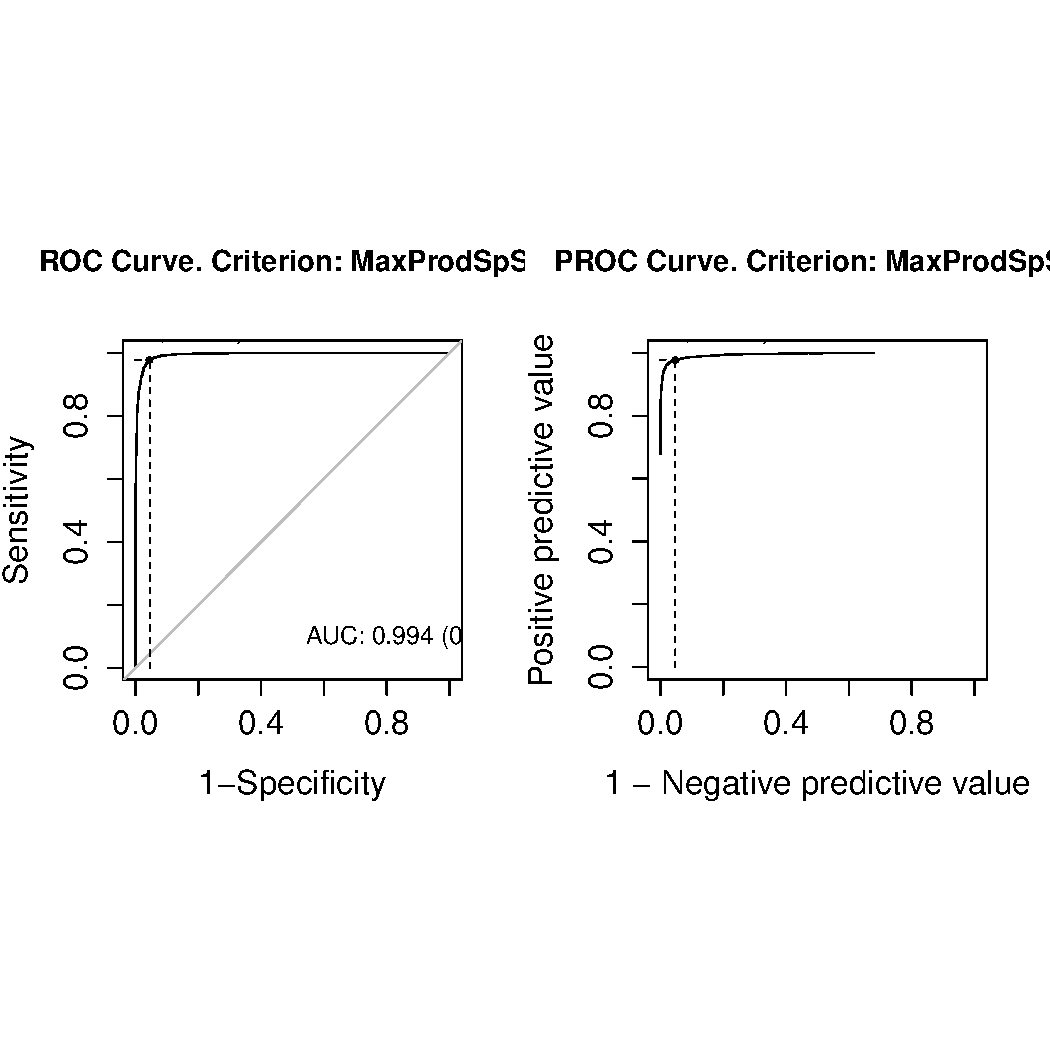
\includegraphics[scale=.49]{roc_left_eye_inner_corner.pdf}
  \label{fig:roc_left_eye_inner_corner}
\end{figure}

\begin{figure}[!htb]
  \centering
  \caption{ROC Curve For Left Eye Center Feature}
  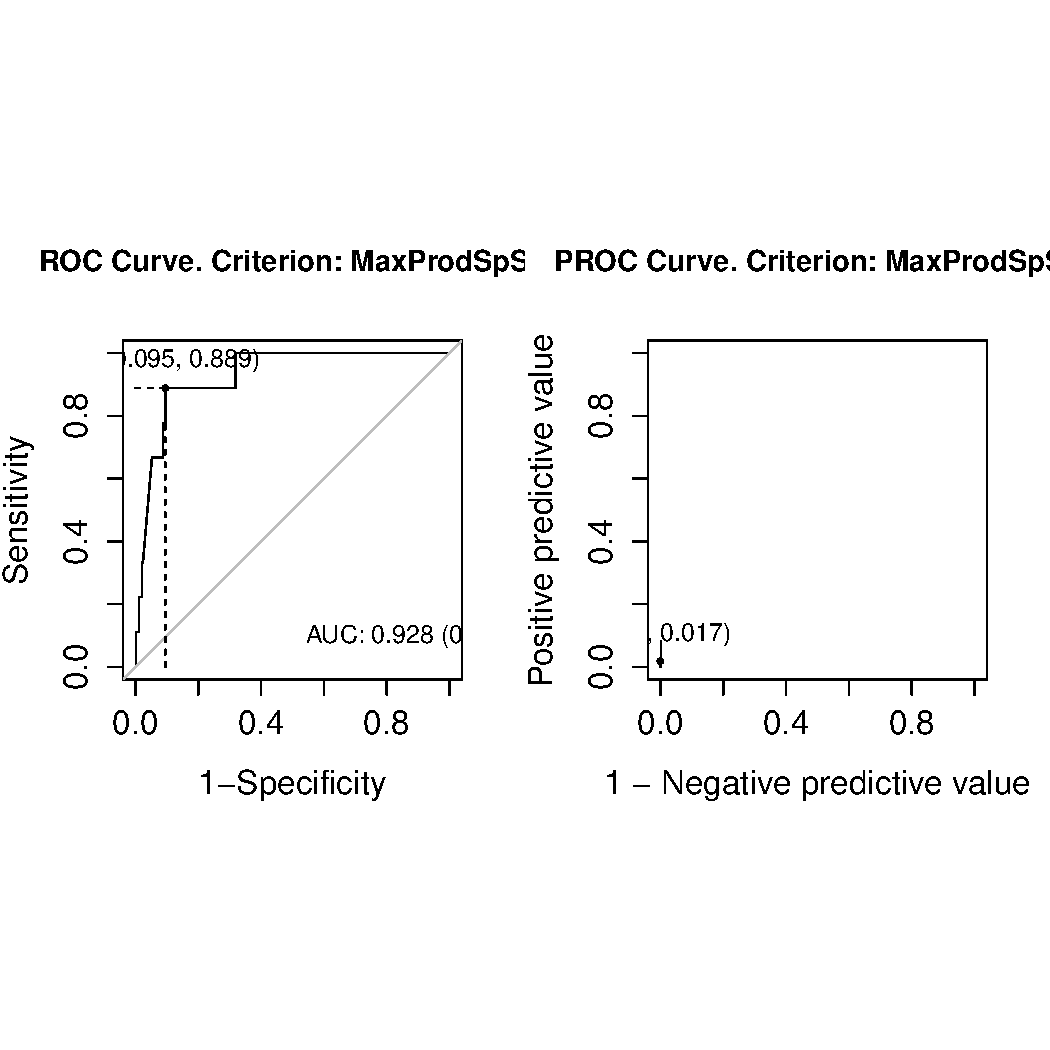
\includegraphics[scale=.49]{roc_left_eye_center.pdf}
  \label{fig:roc_left_eye_center}
\end{figure}

% latex table generated in R 3.2.2 by xtable 1.7-4 package
% Wed Dec  9 11:55:32 2015
\begin{table}[ht]
\centering
\caption{Cutoff Validation Performance} 
\label{tab:logistic_cutoff_table}
\begin{tabular}{lrrr}
  \hline
Feature & Cutoff & Sensitivity & Specificity \\ 
  \hline
Left Eye Center & 0.500 & 0.000 & 1.000 \\ 
  Right Eye Center & 0.500 & 0.000 & 1.000 \\ 
  Left Eye Inner Corner & 0.500 & 0.961 & 0.714 \\ 
  Right Eye Inner Corner & 0.500 & 0.962 & 0.715 \\ 
  Left Eye Outer Corner & 0.500 & 0.960 & 0.713 \\ 
  Right Eye Outer Corner & 0.500 & 0.961 & 0.715 \\ 
  Left Eyebrow Inner End & 0.500 & 0.961 & 0.714 \\ 
  Right Eyebrow Inner End & 0.500 & 0.961 & 0.716 \\ 
  Left Eyebrow Outer End & 0.500 & 0.963 & 0.713 \\ 
  Right Eyebrow Outer End & 0.500 & 0.963 & 0.720 \\ 
  Nose Tip & 0.500 &  &  \\ 
  Mouth Left Corner & 0.500 & 0.961 & 0.718 \\ 
  Mouth Right Corner & 0.500 & 0.960 & 0.716 \\ 
  Mouth Center Top Lip & 0.500 & 0.960 & 0.717 \\ 
  Mouth Center Bottom Lip & 0.500 & 0.000 & 1.000 \\ 
   \hline
\end{tabular}
\end{table}



\section{Individual Keypoint Models}\label{neural}

In this section we will present a subset of the models we experimented with and report performance statistics for each. We will also discuss some auxiliary modeling techniques that we investigated. For each of the models we discuss below, we use a rectifier nonlinear activation and adjust the learning rate and momentum dynamically (discussed in detail below). 

\subsection{Baseline Model}

Our baseline model is a neural network with six layers: 3 convolutional/pooling layers, and 3 hidden layers. We began our modeling with only three layers, but following \cite{benlecun2007}, our idea was that by increasing the depth of the network, we would increase its predictive accuracy as well. Additional layers should, in theory, allow the network to discover or learn more than just the low-level features of the images and hopefully increase its ability to identify specific keypoints.

The hope for the convolutional layer is that it would allow the network to automatically train 2-dimensional filters.  The hope is that the neural network will automatically adapt the filter taps to detect low-level features like edges.  It's possible also that higher-level features (like eyes, noses, mouths) might be trained as well.

The loss function on the validation data set for this set of models is displayed in \cref{fig:val_loss_default}. The RMSE on the validation set is 3.85 (see \cref{tab:model_rmse}).

\begin{figure}[!htb]
  \centering
  \caption{Validation Loss for Feature Detection Models (Baseline)}
  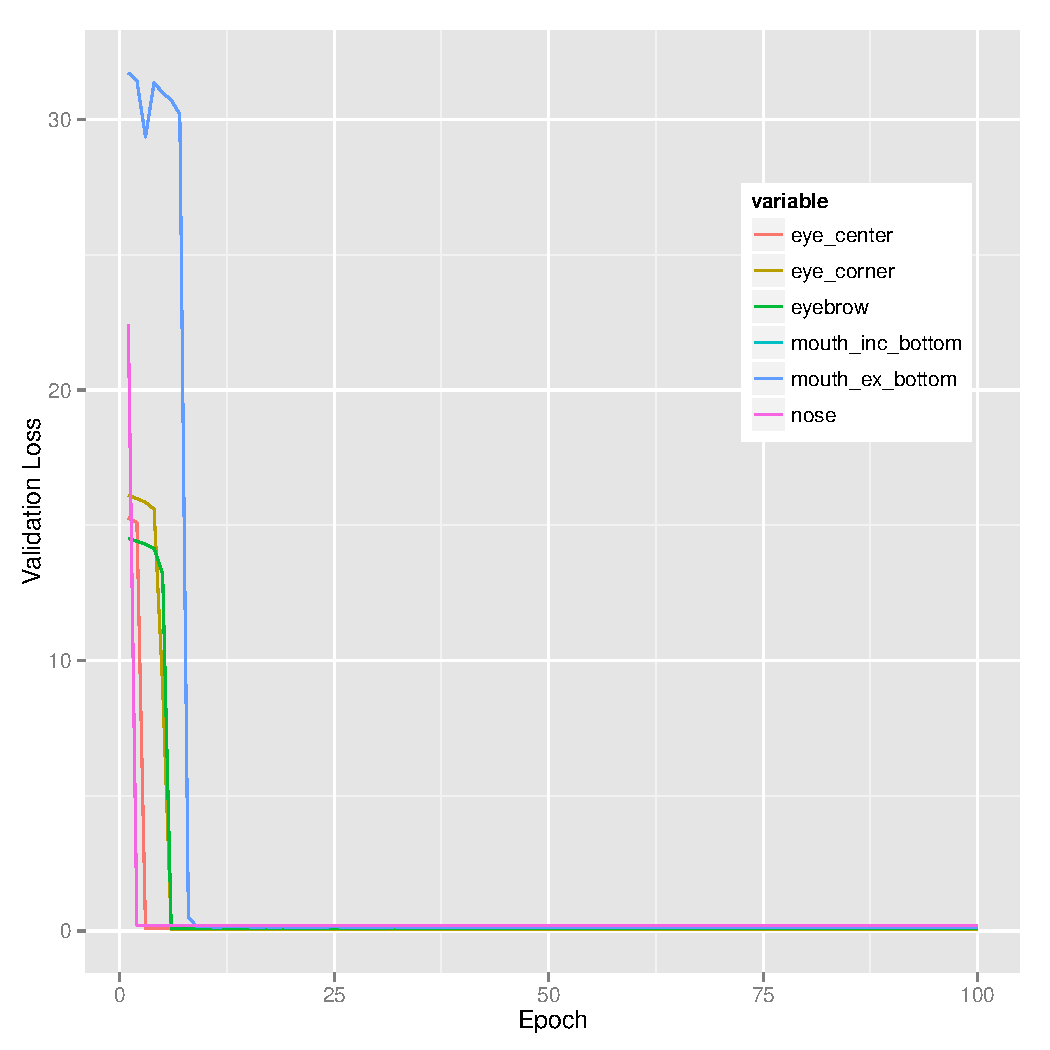
\includegraphics[scale=.49]{val_loss_default.pdf}
  \label{fig:val_loss_default}
\end{figure}

\subsection{Baseline Model with L1 and L2 Regularization}

We augmented our baseline model (described above) with L1 and L2 regularization. Compared to the model without regularization, we find that the loss function falls more gradually and more smoothly. This is because the cost function now has a second term that penalizes model complexity, so that early on in the training cycle the model is less able to fit the data. By not over-fitting the data, the hope is that the model is better at understanding images that it has not seen before. In other words, we are hoping to move the model more towards the optimal trade-off between bias and variance.

The loss function on the validation data set for this set of models is displayed in \cref{fig:val_loss_default_w_l1_and_l2}. The RMSE on the validation set is in excess of 35 (see \cref{tab:model_rmse}), making it far and away our worst performing model. One explanation is that the model has been over-regularized; we have put too much of a premium on building a simple model, so that the result is very bad predictive capability. We can see this a bit in \cref{fig:val_loss_default_w_l1_and_l2}, as the loss function for three of the feature models are not able to stabilize even after 100 epochs.\footnote{We show the results here for 100 epochs; we trained some models for up to 1000 epochs but saw no performance improvements.}

\begin{figure}[!htb]
  \centering
  \caption{Validation Loss for Feature Detection Models (Baseline with Regularization)}
  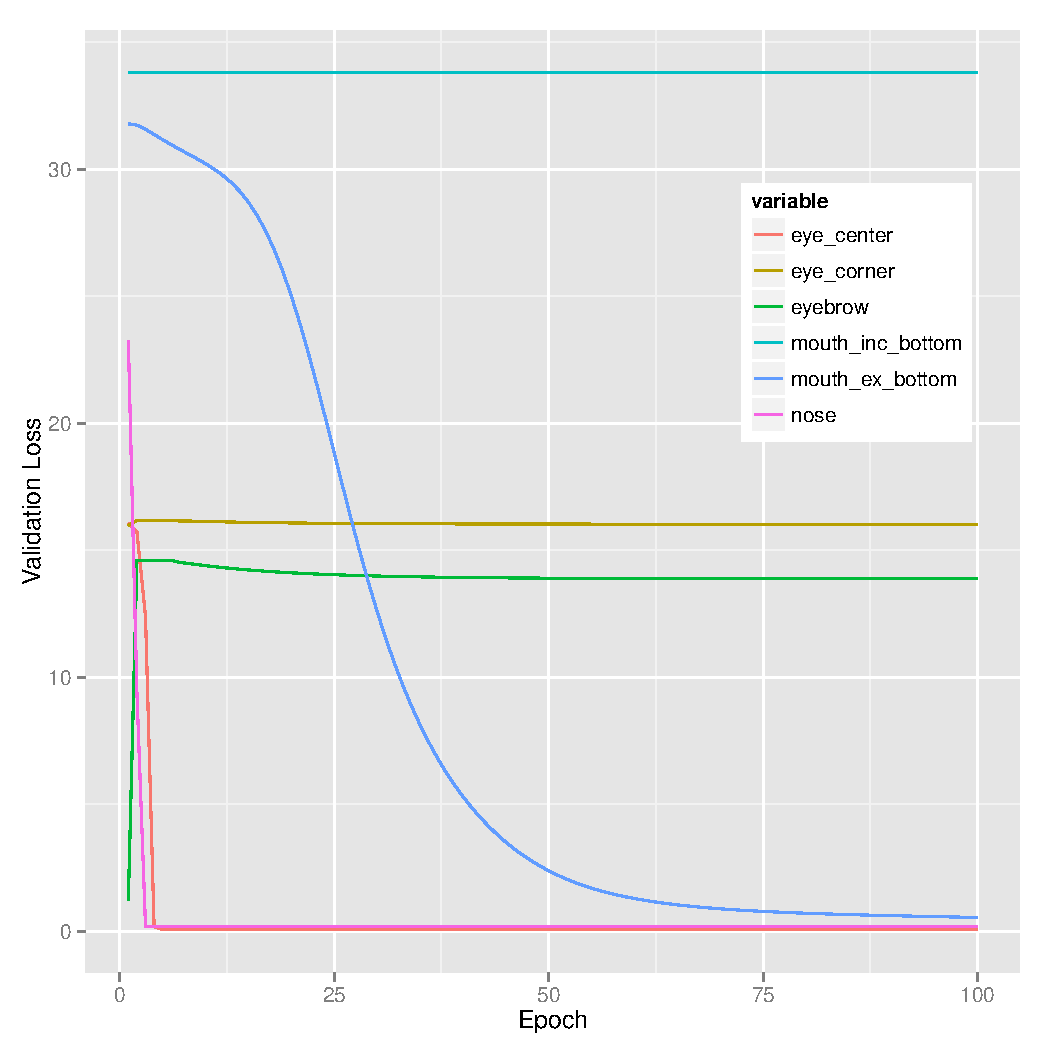
\includegraphics[scale=.49]{val_loss_default_w_l1_and_l2.pdf}
  \label{fig:val_loss_default_w_l1_and_l2}
\end{figure}

\subsection{Inverted Hourglass}

We coined the term inverted hourglass as we explored different neural network structures.  In this model we decided to place more convolutional filters near the input to see if it would improve over our existing model.  Therefore, we essentially flipped the convolutional part of our initial model over (hence the inverted part of the name) to start with 32 filters at the beginning and whittling this down to eight just before the densely connected layer.  Having a much smaller set of filters at the output of the convolutional layer meant that we would use a smaller initial dense layer, which we then doubled and halved again before the output layer (hence the hourglass part).

The loss function on the validation data set for this set of models is displayed in \cref{fig:val_loss_6_level_inverted_hourglass}. The RMSE on the validation set is 3.70, making it our best performing model (see \cref{tab:model_rmse}).

\begin{figure}[!htb]
  \centering
  \caption{Validation Loss for Feature Detection Models (Inverted Hourglass)}
  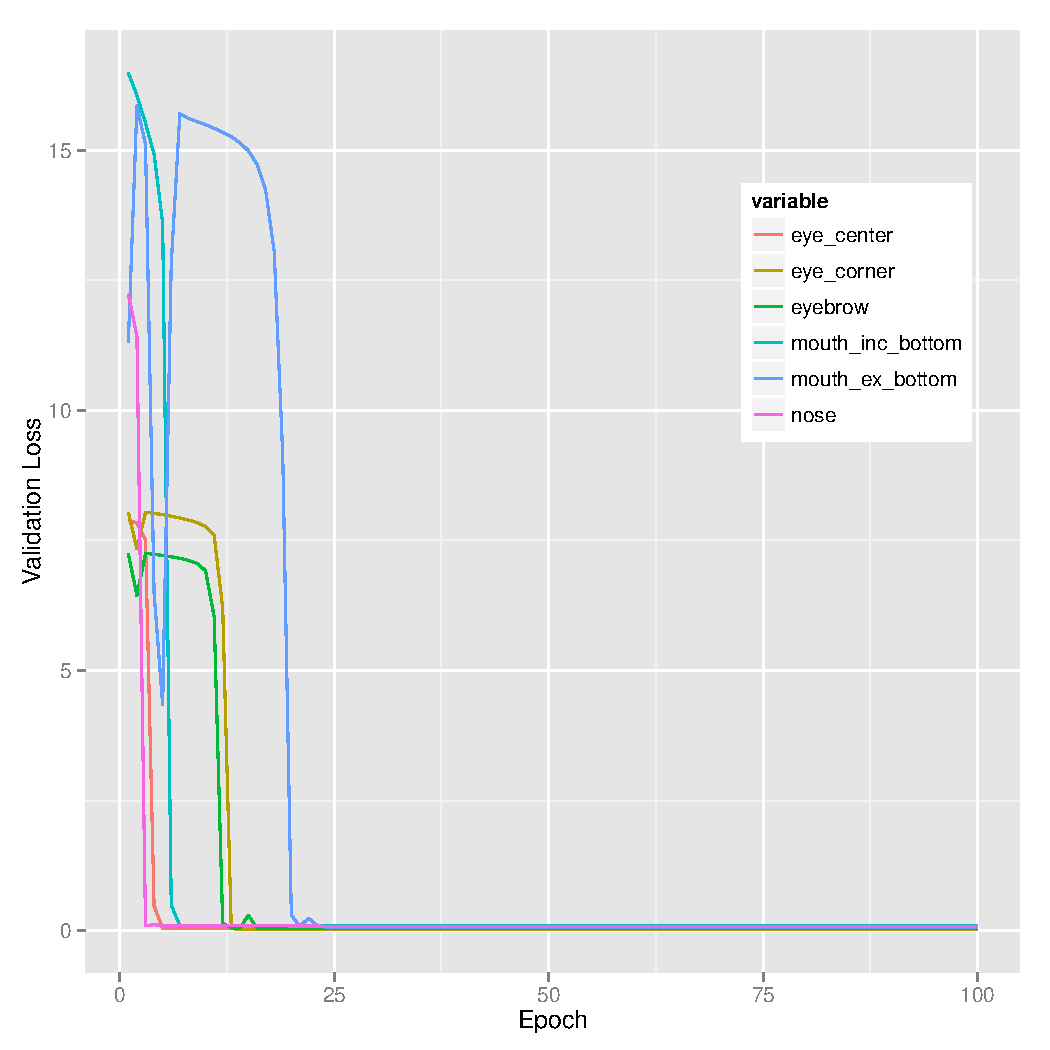
\includegraphics[scale=.49]{val_loss_6_level_inverted_hourglass.pdf}
  \label{fig:val_loss_6_level_inverted_hourglass}
\end{figure}

\subsection{Inverted Hourglass with Regularization}

We augmented our six layer model described above to include only the L1 regularization described above. Once again, the goal here is to prevent the model from over-fitting to the images that it trains on, so penalizing model complexity should increase the out-of-sample accuracy. Following \cite{ng2004feature}, we chose L1 regularization because we have a dimensionally large input data set (each image has 96x96 pixels, with each pixel being an input feature). 

The loss function on the validation data set for this set of models is displayed in \cref{fig:val_loss_6_level_inverted_hourglass_reg}. The RMSE on the validation set is 3.98; predictive performance has declined by adding regularization.

\begin{figure}[!htb]
  \centering
  \caption{Validation Loss for Feature Detection Models (Inverted Hourglass with Regularization)}
  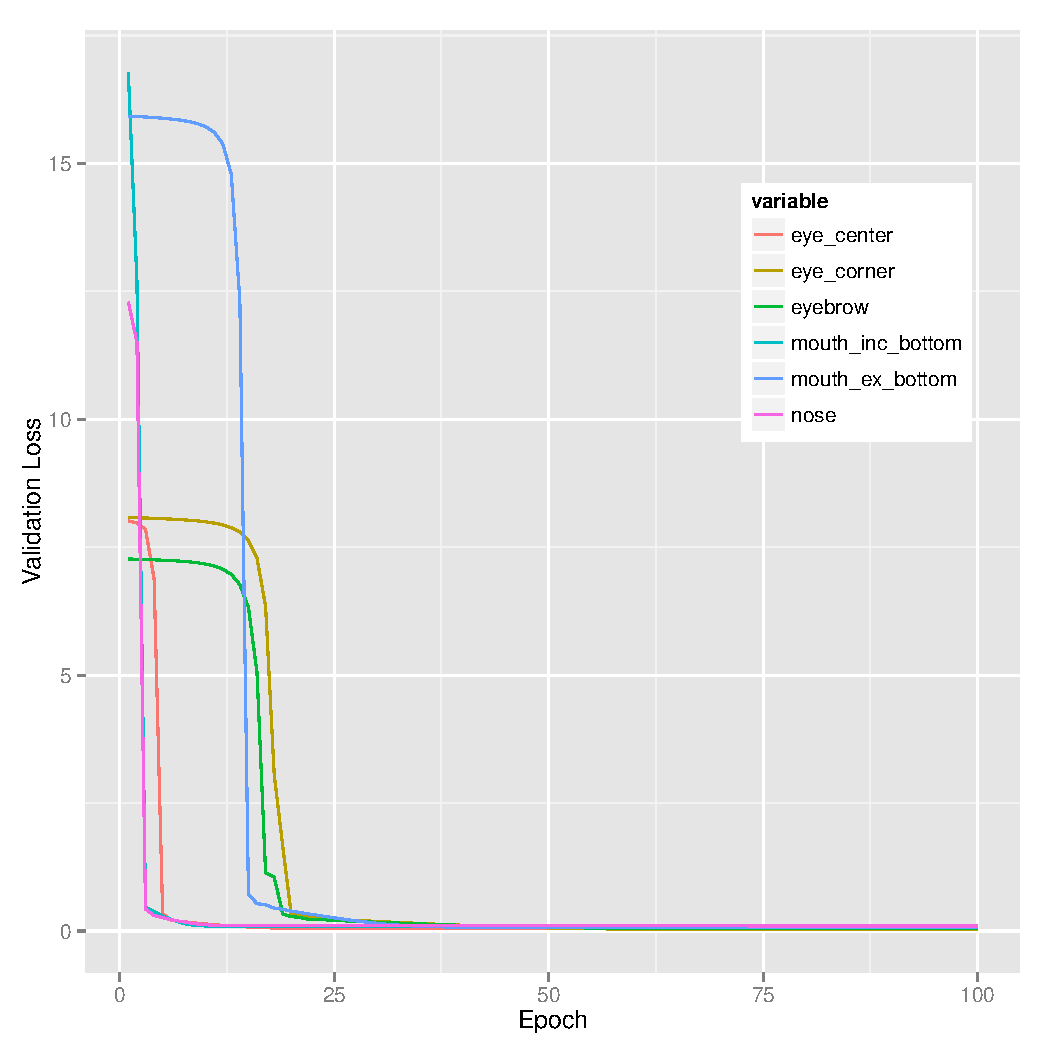
\includegraphics[scale=.49]{val_loss_6_level_inverted_hourglass_reg.pdf}
  \label{fig:val_loss_6_level_inverted_hourglass_reg}
\end{figure}

\subsection{Inverted Hourglass with Regularization and Dropout}

Finally, we further augmented our six layer model with L1 regularization to also include dropout. Similar to regularization, drop helps us ensure that we're not focusing too much on the training set, trying to find the real underlying structure.  Again, the goal is to choose a simpler model, but instead of adjusting the cost function we instead alter the structure of the network by deleting nodes in the intermediate layers during training.

The loss function on the validation data set for this set of models is displayed in \cref{fig:val_loss_6_level_inverted_hourglass_reg_do}. The RMSE on the validation set is 4.40; predictive performance has declined again by combining dropout with regularization.

\begin{figure}[!htb]
  \centering
  \caption{Validation Loss for Feature Detection Models (Six Layers)}
  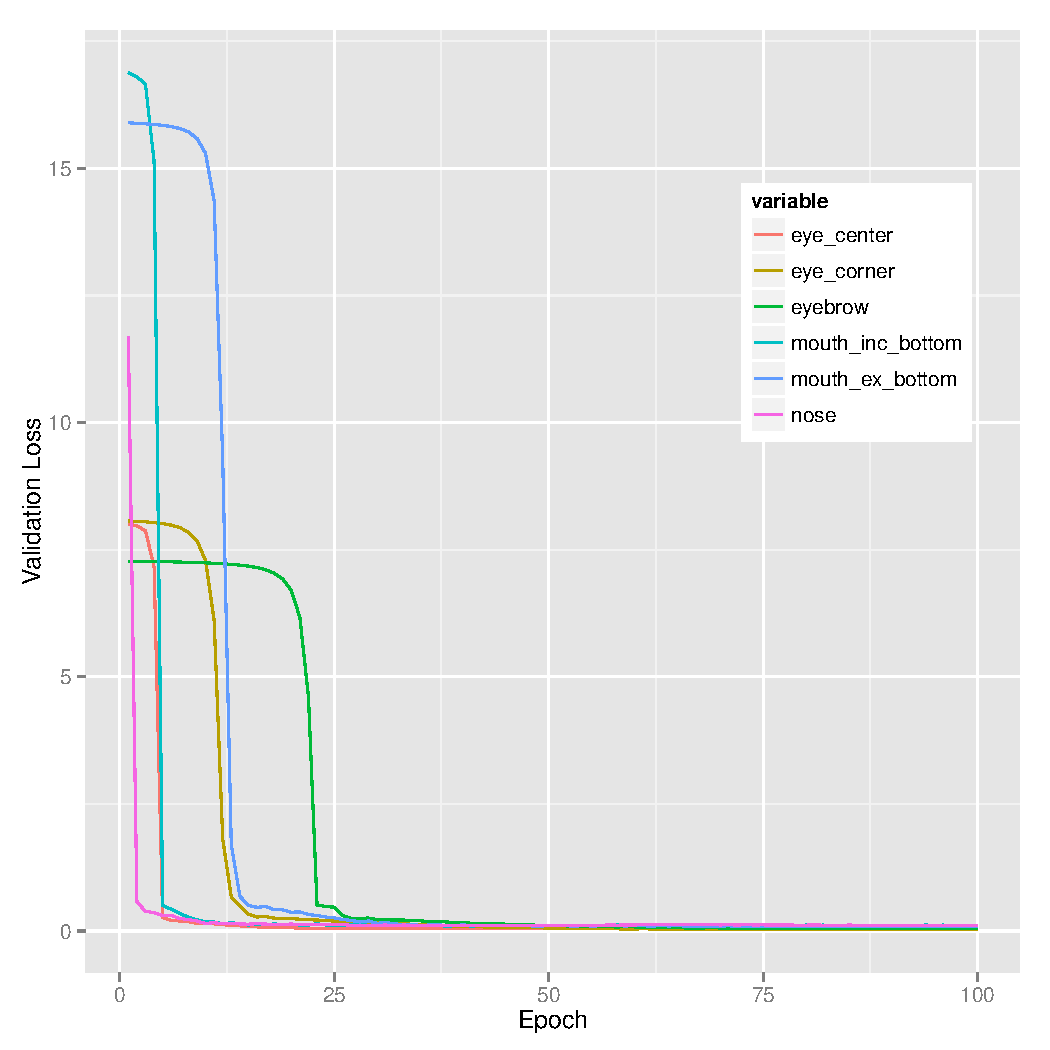
\includegraphics[scale=.49]{val_loss_6_level_inverted_hourglass_reg_do.pdf}
  \label{fig:val_loss_6_level_inverted_hourglass_reg_do}
\end{figure}

% latex table generated in R 3.2.2 by xtable 1.7-4 package
% Thu Dec 10 16:07:50 2015
\begin{table}[ht]
\centering
\caption{RMSE for Different Model Structures} 
\label{tab:model_rmse}
\begin{tabular}{lr}
  \hline
Model & RMSE \\ 
  \hline
Inverted Hourglass & 3.70 \\ 
  Inverted Hourglass with Regularization & 3.98 \\ 
  Inverted Hourglass with Regularization, Dropout & 4.40 \\ 
  Baseline & 3.85 \\ 
  Baseline with Regularization & 35.21 \\ 
   \hline
\end{tabular}
\end{table}


\subsection{Other Modeling Choices}

After being somewhat displeased with the results, we tried many other methods to see if we could train the model a bit better.  These experiments included and discussed in the following subsections.

\subsubsection{Batch-Size}
While batch-size shouldn't really matter, we did want to see if it had any effect on the training.  As it turns out, we did notices that larger batch-sizes did help lower the resulting RMSE slightly.  This was likely because the nesterov momentum update algorithm could incorporate a larger amount of the data-set in each update.

\subsubsection{Learning-Rate}
When we initially set the learning rate too high, we quickly saturated our 32-bit floating-point accumulators (GPUs can only handle single-precision floating point operations). Additionally, we knew that if we set it too low, we would wait forever to converge to an answer and, worse-yet, risked ending up in a local minima.

We had to balance setting it too high and too low.  After some consideration we saw that dynamic learning-rates were common-place \cite{gorr,dnouri} and we opted to implement and experiment with both a log and a linear learning-rate backoff based, for simplicity, solely on the number of epochs trained.

\subsubsection{Momentum}
Our update algorithm (nesterov updates) included both a learning-rate and momentum parameter.  After reading a bit in \cite{gorr} about the advantages of momentum in the overall amount of time needed to train a network we set about determining a reasonable value.  Further reading in the lasagne manual \cite{lasagnenesterov} led us to experiment not only with static momentum parameters but also with dynamic ones that increased momentum as learning-rate decreased.

\subsubsection{Dropout}
We played a bit with varying the amount of dropout present in the network.  We found that too little and too much dropout had, unsurprisingly, negative effects on the training.  In the former case, we likely were over-fitting our data, in the latter one, we introduced too much noise to train on.  We found that 10-20\% dropout was appropriate for our network.

\subsubsection{Scaling Output}
Finally, in an effort to see if we could get the neural network to train a little better, we tried scaling the output to lie between -1 and 1 in one experiment.  In another we tried normalizing it to so that coordinate positions were measured in standard deviations away from the mean.  Unfortunately we did not see improvements in the RMSEs produced by either of these experiments (reported training RMSEs were higher since the scale was smaller, but the resulting de-scaled RMSEs were worse).

\subsection{Image Pre-processing}

One key observation of our models outputs is that most of the predicted keypoints are very close to the average location of each keypoint. That is, to a first approximation our models just predict a keypoint will be at its average location; the variance is possibly due to the model learning to understand localized variation in the images.

One idea to help the model learn the ``true'' features of each face would be to pre-process the images by rotating them. Our goal would be that the model could not simply predict average locations for each keypoint, but would have to truly learn what signals the location of an eye, or a nose, etc. 

To implement this, we augmented the training data set with 3 copies of each image, rotated 90, 180, or 270 degrees. Unfortunately, the results did not meet our expectations, as the RMSE of the model trained on the augmented data set exceeded the RMSE of the baseline model by at least 2 times. It appeared as though the model was still, to a first approximation, predicting the average location of each keypoint, although because the images were rotated, the average location was nowhere close to the actual location for any of the images.

\subsection{Learning Representation}

We also tried using the penultimate layer of our baseline neural network as the input into a different type of model (random forest or penalized regression, in our case). The idea is to use the neural network to learn and identify important features of the data, and then to use these important features in a final predictive model. Unfortunately, this methodology did not produce successful results in our case. The RMSE produced by this additional layer of modeling was worse than the traditional baseline model, so we did not investigate it any further.

\subsection{Combined Model}

In the combined model, we attempted to train both the missing data probability and the feature coordinate locations simultaneously.  This involved a fair amount of additional work to better understand the inner-workings of Theano and Lasagne, but the idea was that if we could train both models at once, we wouldn't have to train 7 models in total (6 feature-sets + the missing probability).  Additionally, because the neural network had to detect the presence of the missing feature, it was hoped it could use this to predict location better. Finally because the neural network could see all images in the training dataset, it could theoretically do a better job learning.  To do this, we had to create a loss-function that combined RMSEs from the keypoint coordinates and Binary-Cross-Entropy values from the logistic output.  To make matters more complicated, we had to write this loss-function to not penalize the network for a coordinate given on a missing feature.  Unfortunately, when the model was built and run, it fared worse than the model trained on the 7 separate features. It is likely that a better loss-function could have helped this, but due to time-constraints we were forced to move-on.

\section{Discussion}

\subsection{Best and Worst Performances}

In \cref{fig:avg_face_rmse}, we show an ``average'' face, i.e., one that is a composite of all images in our data set. On the image is the average location of each keypoint (marked with a ``+'' sign), and the shaded circles show the average deviation of the predicted keypoints from the actual keypoints. Colors correspond to the model used for each set of keypoints (i.e. eye corners were all predicted with one model, so they are all depicted in yellow).

We can consider the accuracy of our model in two different ways: the RMSE of each keypoint coordinate (shown in \cref{tab:rmse}), or the Euclidean distance of the predicted keypoint $(x,y)$ coordinate from the actual $(x,y)$ coordinate (shown in \cref{tab:rmse}; these are represented by the circles in \cref{fig:avg_face_rmse}). 

From the distances between predicted in actual keypoints in \cref{tab:radius}, we can see that the model is best at predicting eye features. The top of the list (ordered from most to least accurate) is comprised entirely of the eye-related features (eye centers, eye corners, and eyebrows). We can see in \cref{fig:avg_face_rmse} that the radii around the eye features are smaller than those of the nose and mouth features. The most accurate keypoint is the inner corner of the right eye, which has a distance between the predicted and actual keypoints of just over three pixels.

Conversely, the model is not very good at predicting where the tip of a nose is. It is the least accurate keypoint, with a mean distance between the predicted and actual value of over six pixels.

% latex table generated in R 3.2.2 by xtable 1.7-4 package
% Wed Dec  9 12:53:27 2015
\begin{table}[ht]
\centering
\caption{RMSE for Predicted Keypoints} 
\label{tab:rmse}
\begin{tabular}{lr}
  \hline
Keypoint & RMSE \\ 
  \hline
right eye inner corner x & 2.46 \\ 
  mouth center top lip x & 2.48 \\ 
  right eye inner corner y & 2.57 \\ 
  right eyebrow inner end y & 2.68 \\ 
  left eye inner corner y & 2.70 \\ 
  right eyebrow inner end x & 2.71 \\ 
  left eyebrow inner end y & 2.72 \\ 
  right eye outer corner y & 3.04 \\ 
  left eyebrow inner end x & 3.05 \\ 
  left eye outer corner y & 3.07 \\ 
  right eye outer corner x & 3.17 \\ 
  mouth left corner x & 3.26 \\ 
  left eyebrow outer end y & 3.29 \\ 
  right eye center x & 3.37 \\ 
  right eyebrow outer end y & 3.38 \\ 
  right eyebrow outer end x & 3.39 \\ 
  mouth right corner x & 3.42 \\ 
  left eye inner corner x & 3.48 \\ 
  right eye center y & 3.50 \\ 
  left eye center y & 3.57 \\ 
  left eyebrow outer end x & 3.59 \\ 
  left eye center x & 3.75 \\ 
  left eye outer corner x & 4.01 \\ 
  mouth right corner y & 4.29 \\ 
  mouth center bottom lip x & 4.32 \\ 
  nose tip x & 4.34 \\ 
  mouth left corner y & 4.62 \\ 
  mouth center top lip y & 5.22 \\ 
  mouth center bottom lip y & 5.60 \\ 
  nose tip y & 5.91 \\ 
   \hline
\end{tabular}
\end{table}

% latex table generated in R 3.2.2 by xtable 1.7-4 package
% Wed Dec  9 12:52:05 2015
\begin{table}[ht]
\centering
\caption{Average Euclidean Distance between Predicted and Actual Keypoints} 
\label{tab:radius}
\begin{tabular}{lr}
  \hline
Keypoint & Average Distance \\ 
  \hline
right eye inner corner & 3.17 \\ 
  right eyebrow inner end & 3.32 \\ 
  left eyebrow inner end & 3.55 \\ 
  right eye center & 3.57 \\ 
  right eye outer corner & 3.89 \\ 
  left eye inner corner & 3.96 \\ 
  left eye center & 3.97 \\ 
  right eyebrow outer end & 4.10 \\ 
  left eyebrow outer end & 4.18 \\ 
  left eye outer corner & 4.43 \\ 
  mouth right corner & 4.74 \\ 
  mouth left corner & 4.82 \\ 
  mouth center top lip & 4.91 \\ 
  mouth center bottom lip & 5.82 \\ 
  nose tip & 6.07 \\ 
   \hline
\end{tabular}
\end{table}


\subsection{Model Evaluation}

One baseline to judge model performance is how well we predict relative to naive averaging of keypoints. That is, one simple algorithm would be to predict--for all faces in the data set--the average of each keypoint across all faces. Doing so yields an average RMSE (across all keypoints) of 3.6. This actually compares favorably to the predictive capability of our best model, which produces an RMSE of 3.7. It appears that the model configurations we experimented with were not able to truly learn the features of facial keypoints. 

One feature that stands out when examining the badly mis-predicted faces in \cref{fig:worst_faces} is that the model tends to predict keypoints close to their average values regardless of how the face in a given image is oriented. We can see this playing out in the plots above showing the validation losses for each model; in most cases, the validation loss relatively quickly drops then stays constant for the remainder of the training run. One interpretation of this is that the model quickly learns where the average keypoints are on an image, then fails to learn any other features of the data sets. It is possible that there are too few exemplars with tilted faces for the model to train against and thus it does a relatively poor job with these features.

\begin{figure}[!htb]
  \centering
  \caption{Average Face with Estimated Keypoints}
  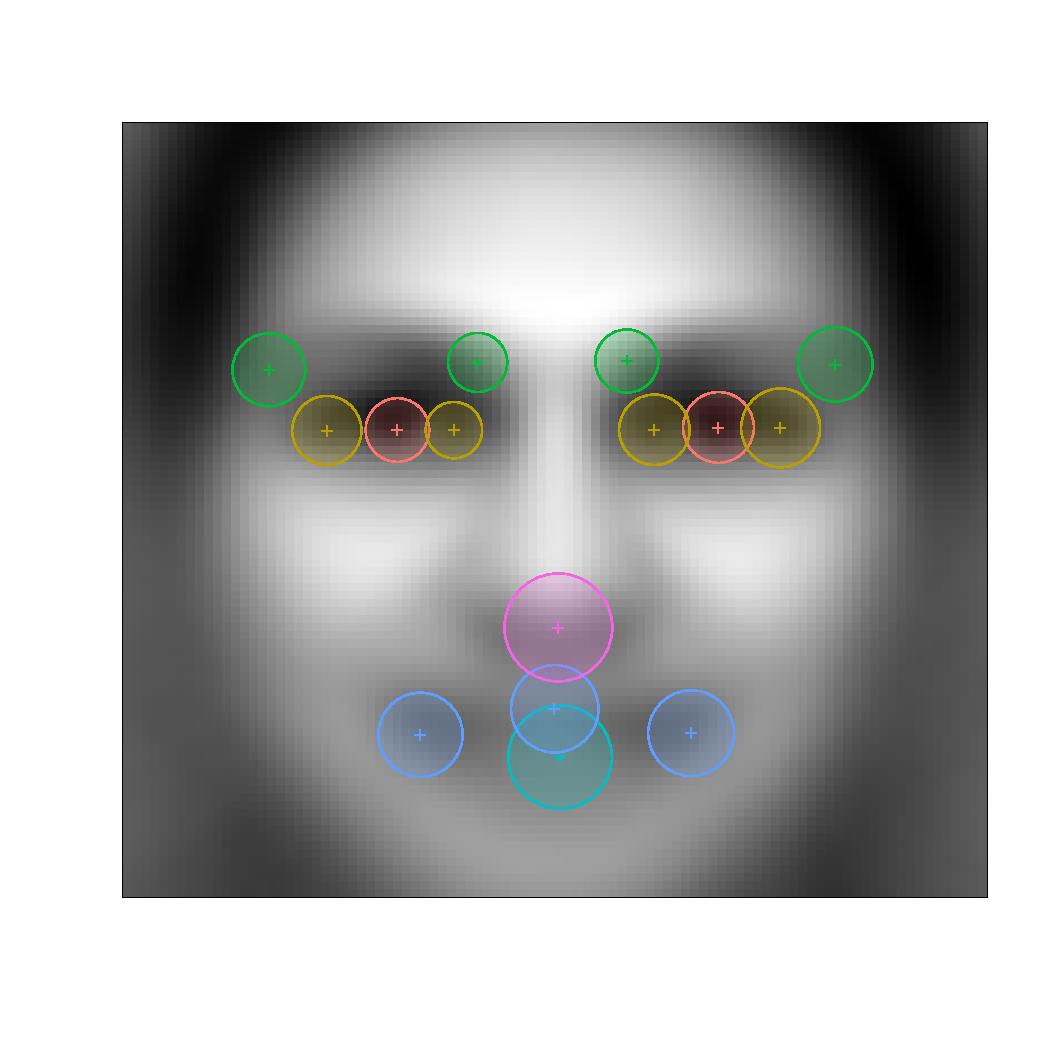
\includegraphics[scale=.49]{avg_face_rmse.pdf}
  \label{fig:avg_face_rmse}
\end{figure}

\begin{figure}[!htb]
  \centering
  \caption{Most Accurate Predictions (Average RMSE = 1.768764)}
  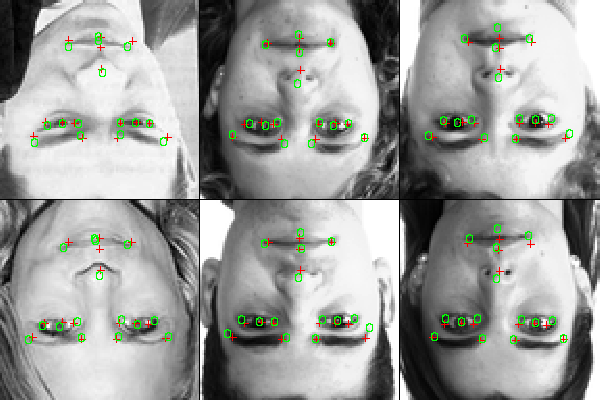
\includegraphics[scale=.49]{best_faces.pdf}
  \label{fig:best_faces}
\end{figure}

\begin{figure}[!htb]
  \centering
  \caption{Least Accurate Predictions (Average RMSE = 7.874467)}
  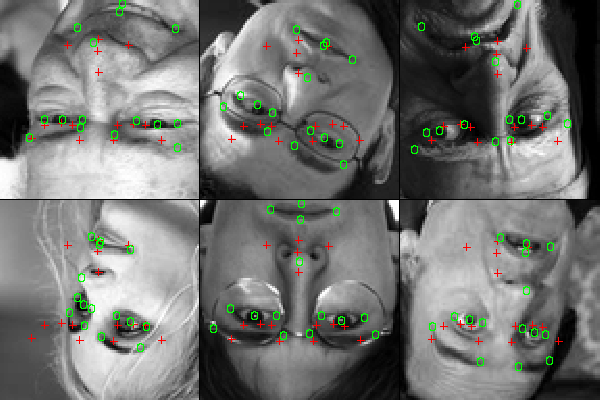
\includegraphics[scale=.49]{worst_faces.pdf}
  \label{fig:worst_faces}
\end{figure}

\section{Kaggle Submission}

As a final and true out-of-sample test, we used the model with the best RMSE on the validation data set (the Inverted Hourglass model) to predict on the Kaggle test set. This is a set of 1783 images for which we know the pixel values but not the true keypoint values. The only way to judge the accuracy of the model on this set is to submit results to Kaggle. Our submission was graded to have an RMSE of 4.16987, which at the time of this writing puts us in 105th place. The RMSE of this submission is significantly higher than our validation RMSE. One possibility is that the training set is different than the testing set, as the training set is composed of images without all keypoints while the testing set is composed of images with all keypoints labeled, suggesting they are perhaps from different sources. Another possibility is that our model has over-trained on the training set, but given the relatively high validation RMSE we suspect this is not likely.

\bibliographystyle{IEEEtran}
\bibliography{citations}

\end{document}

% \input{.tex}

% \begin{figure}[!htb]
%   \centering
%   \begin{subfigure}[b]{0.49\textwidth}
%     \caption{}
%     \includegraphics[width=\textwidth]{.pdf}
%     \label{fig:}
%   \end{subfigure}
%   \hfill
%   \begin{subfigure}[b]{0.49\textwidth}
%     \caption{}
%     \includegraphics[width=\textwidth]{.pdf}
%     \label{fig:}
%   \end{subfigure}
%   \caption{}
% \end{figure}

% \begin{figure}[!htb]
%   \centering
%   \caption{}
%   \includegraphics[scale=.49]{.pdf}
%   \label{fig:}
% \end{figure}